\chapter{Introduction}

Heads-Up Displays (HUDs) have been used for many years in fighter jets and
large airliners. These displays provide pilots with many important metrics.
Information is displayed in the pilot's field of view so that he or she
does not have to look down at the aircraft gauges, hence the name
``heads-up.'' In addition, the display is also focused at infinity. This
allows the pilot to keep his or her eyes focused on the real world while
still viewing important information.

\begin{figure}[h]
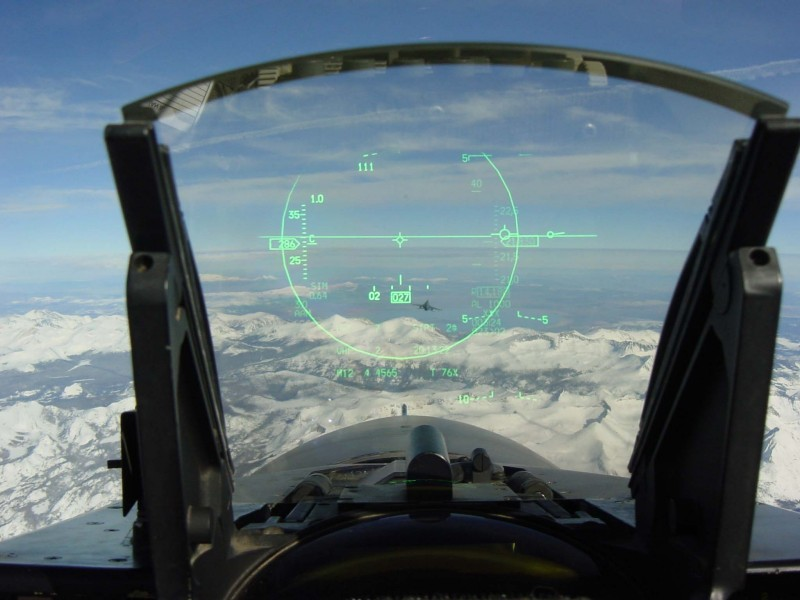
\includegraphics[width=\textwidth]{img/JetHUD.jpg}
\caption{A HUD shown in a fighter jet}
\label{fig:jetHUD}
\end{figure}

The two main properties of HUDs (i.e. being focused at infinity and being
in the field of view) provide advantages over traditional displays. Since
the display is ``heads-up,'' the pilot does not need to waste time looking
down at gauges or dash mounted displays. Even if these displays were in the
down at gauges or dash mounted displays. Even if these displays were in the
field of view, they would still not be very useful since the pilot would
have to refocus from the real world (essentially infinity) to the displays
(approximately one meter) and then back again. This focusing/refocusing
process can potentially be very disorienting. While these may seem trivial,
these operations could be deadly at several hundred meters per second.
Figure~\ref{fig:jetHUD} shows an image of the HUD from an FA-18 ``Hornet''
fighter jet.

While the stakes are much lower in automobiles, HUDs can still greatly
enhance driver experience. Car metrics such as speed, engine RPM, fuel
level, and direction can be displayed in much the same way as is done in
aircraft. This allows the driver to keep his eyes on the road and other
vehicles. There have even been efforts to display augmented reality
information such as ``night vision'', lane detection, and obstacle detection
into the driver's field of view.

HUDs have been used in automobiles for a number of years and have become
much more popular recently. General Motors began using HUDs in some Pontiac
models and has since extended the technology to Corvettes and other models.
BMW has used HUDs in their E60 models and has begun using multiple color
displays. Many aftermarket options exist as well, although none of them
match the performance of the OEM systems. The following
Figures~\ref{fig:PontiacHUD}--\ref{fig:BMWHUD} illustrate examples of HUDs
in consumer vehicles.

\begin{figure}
	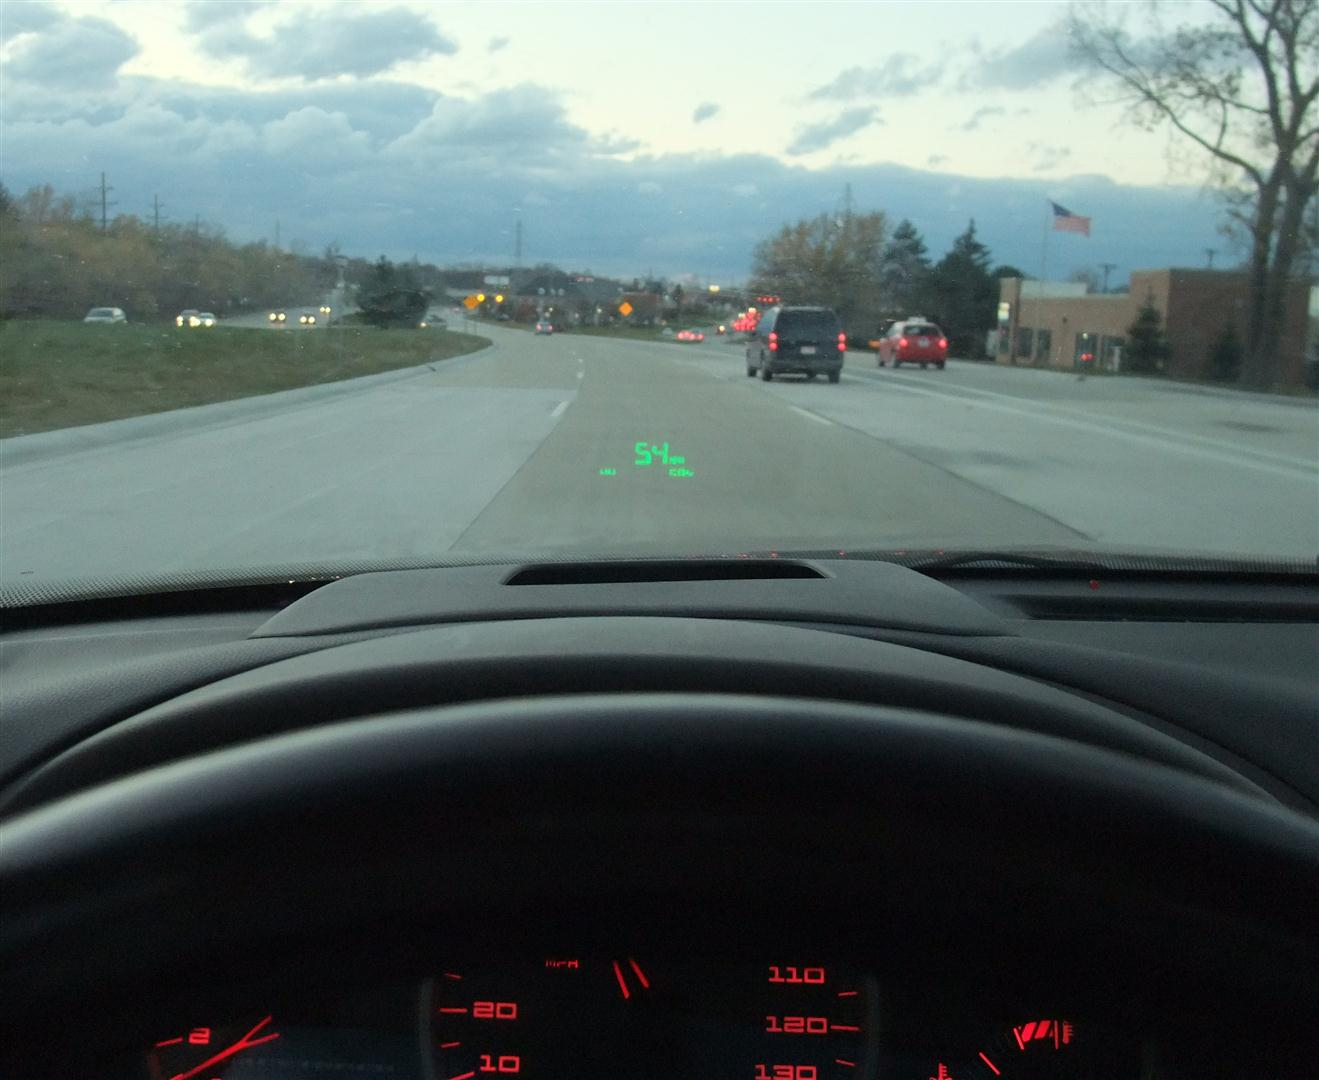
\includegraphics[width=\textwidth]{img/PontiacHUD.jpg}
	\caption{Pontiac HUD}
	\label{fig:PontiacHUD}
\end{figure}

\begin{figure}
	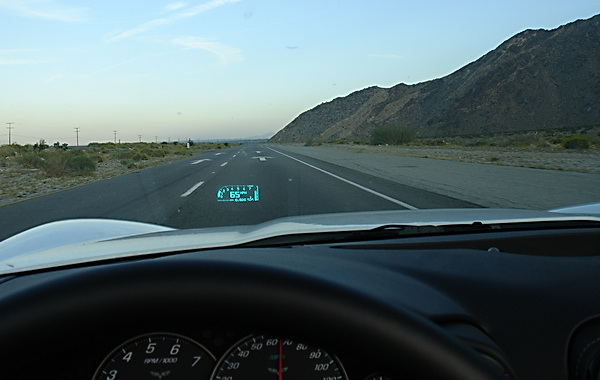
\includegraphics[width=\textwidth]{img/CorvetteHUD.jpg}
	\caption{Chevrolet Corvette HUD}
	\label{fig:CorvetteHUD}
\end{figure}

\begin{figure}
	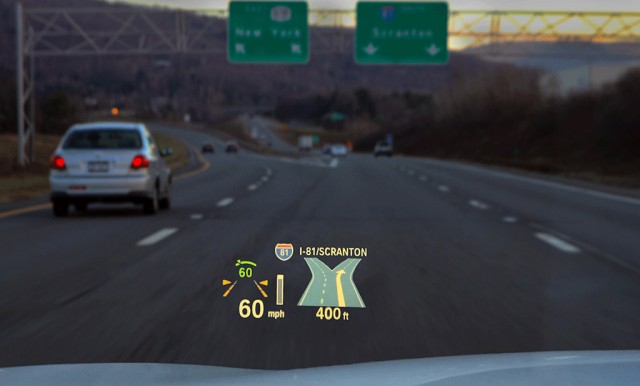
\includegraphics[width=\textwidth]{img/BMWHUD.jpg}
	\caption{BMW HUD}
	\label{fig:BMWHUD}
\end{figure}

Obviously, these displays could be very beneficial to a driver. It is for
this reason the project team wants to develop a display that is (to some
degree) universal. The ability to add a HUD to almost any vehicle could
greatly enhance the driving experience.

Many aftermarket systems currently have the capability to display vehicle
metrics; however it is truly the display portion that is lacking. These
systems cannot focus their displays at infinity. This is certainly due to
costs, but it completely misses the point of a heads-up display. This
project should be able to deliver a product that will not only display
vehicle information but do so in a true heads-up fashion.

The greatest challenge of this project will be developing a display that
can be seen in many lighting conditions. Many modern OEM setups use Vacuum
Fluorescent Displays (VFD) which offer high brightness but are generally
limited to small number of colors. With the advent of Organic LED displays
it may be possible to provide a full color display that is bright enough
for daytime use. Traditional LCD screens are not practical since they rely
on backlights; these are easily overpowered by sunlight.
